

\documentclass[12pt, letterpaper]{report}
\usepackage[utf8]{inputenc}
\usepackage{graphicx}
\graphicspath{ {Downloads/} }



\title {Finite State Machine \\  ID1340 \\Digital System Design}
\author{Shreyas Jayant Havaldar \\  CS18BTECH11042 }
\date{\today}

\begin{document}

\maketitle

\tableofcontents

\begin{abstract}

The objective of this project is to design a finite state machine which will control the car lights according to the live input fed by the user. The car consists of 6 lights which have been depicted as LEDs on the breadboard and the user supplies the input as left, right or hazard. As long as the input is left, the 3 left LEDs light up in sequence followed by IDLE state cyclically. Likewise for right signal 3 right LEDs are lit up followed by IDLE state cyclically. For hazard signal all lights blink simultaneously. 

\end{abstract}

\chapter{Designing The Circuit}
\section{Input Signals}
To take live input from the user we read a character from the serial monitor using the \textit{Serial.read()} function if there is a new character entered by the user. We assign the character entered to a char variable 'x' declared in the arduino code. If there is no new input from the user the previous input signal is continued. \\ 
\textbf{The variables 'P', 'Q' denote the MSB and LSB of the input signal respectively.}


\begin{itemize}


 \item If the user enters 'L': the initial state assigned is that of LA glowing and the user input is assigned to '01'; Left signal is represented by '01' in the code. \textbf{P=0;Q=1;A=0;B=0;C= 1;}
  \item If the user enters 'R': the initial state assigned is that of RA glowing and the user input is assigned to '10'; Right signal is represented by '10' in the code. \textbf{P=1;Q=0;A=1;B=0;C= 0;}
  \item If the user enters 'H': the initial state assigned is that of Hazard Blinking and the user input is assigned to '00'; Hazard signal is represented by '00' in the code. \textbf{P=0;Q=0;A=0;B=0;C= 0;}
  
  
\end{itemize}


 

 
\section{States}
 
We may encounter \textbf{8 different states} in our execution and therefore use \textbf{3 bits} to denote the current state and the next state. Variables W, X, Y represent the current state in execution and A, B, C denote the next state where W and A are the MSBs respectively. We assign the following binary numbers to the each state. 
\\ 
 


\begin{center}
 \begin{tabular}{||c c c c||} 
 \hline\hline
 Physical State & W & X & Y \\  [0.5ex] 
 \hline\hline\hline
 Only LA is glowing & 0 & 0 & 1 \\ 
 \hline
 LA and LB are glowing & 0 & 1 & 0 \\
 \hline
 LA, LB, LC are glowing & 0 & 1 & 1 \\
 \hline\hline
  Only RA is glowing & 1 & 0 & 0 \\ 
 \hline
 RA and RB are glowing & 1 & 0 & 1 \\
 \hline
 RA, RB, RC are glowing & 1 & 1 & 0 \\
 \hline\hline
 No light glowing & 1 & 1 & 1 \\
 \hline\hline
 All lights glowing & 0 & 0 & 0 \\ [1ex] 
 \hline\hline

\end{tabular}

\end{center}





\section{State Transition Diagram}
The drawn state transition diagram is obtained and used to write transition states. 
 \\ \\ \\ \\ \\ \\ \\ \\ \\ \\ \\ \\

  

\begin{figure}
    \centering
    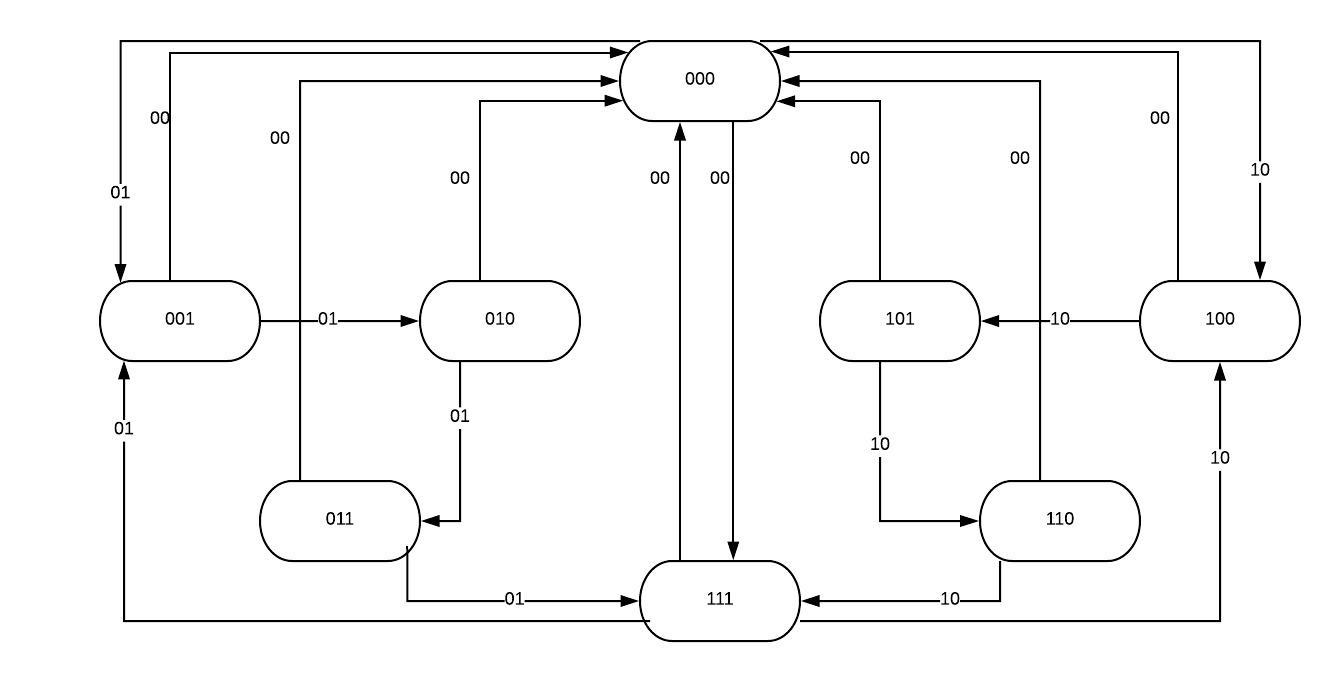
\includegraphics[scale=0.7]{States}
    \caption{State Transition Diagram}
    \label{fig:my_label}
\end{figure}




\section{Incorporating Flip Flops}

We use \textbf{3 D flip-flops} as we encounter $2^3$ states. Each flip-flop is used to transit 1 bit and it takes A, B, C as the 'D' and produces W, X, Y as the 'Q'. We provide A, B, C using Arduino Output pins : 2, 3, 4 and read W, X, Y from the flip-flops using defined Arduino Input pins: 5, 6, 7. The clear and preset of each flip-flop is given 1. \\ \\ \\ \\ \\ \\ \\ \\ \\ \\ \\ \\

\section{Transition Table}

The combined transition table for all possible cases is as follows:


\begin{center}
 \begin{tabular}{||c c c c||} 
 \hline
  & 01 (LEFT) & 10 (RIGHT)  & 00 (HAZARD)  \\ [0.5ex] 
 \hline
 WXY & ABC & ABC & ABC \\ 
 \hline\hline
 001 & 010 & 100 & 000 \\ 
 \hline
 010 & 011 & 100 & 000 \\ 
 \hline
  011 & 111 & 100 & 000 \\ 
 \hline
  100 & 001 & 101 & 000 \\ 
 \hline
 101 & 001 & 110 & 000 \\ 
 \hline
 110 & 001 & 111 & 000 \\ 
 \hline
 111 & 001 & 100 & 000 \\ 
 \hline
 000 & 001 & 100 & 111 \\ 
 \hline
 \hline
 
\end{tabular}
\end{center}

\section{Transition Equations}
For each bit there is a unique transition equation which are as follows:

  \begin{equation}
  A=(P.Q')+(P'.Q.W'.X.Y)+(P'.Q'.W'.X'.Y')
  \end{equation}
 

 
  \begin{equation}
  B= (P.Q'.W.X'.Y)+(P.Q'.W.X.Y')+((P'.Q.W').(X+Y))+ (P'.Q'.W'.X'.Y')
  \end{equation}
 
  \begin{equation}
  C=((P'.Q).(( W'.X'.Y)'))+(P.Q'.W.Y)+(P'.Q'.W'.X'.Y')
  \end{equation}
  





\chapter{Implementation}

\section{Hardware Requirements}

The hardware that was required to complete this project is:



\begin{enumerate}
  \item Arduino UNO
  \item USB A to USB B Adapter
  \item Breadboard
  \item 2 7474 ICs
  \item 6 LEDs
  \item 6 Resistors
  \item Connecting Wires
  
\end{enumerate}



\section{Giving output to LEDs}

Each LED should light up corresponding to the required state. Therefore we use 6 output pins from the arduino: 8, 9, 10, 11, 12, 13 corresponding to LC, LB, LA, RA, RB, RC respectively. 

\begin{center}
 \begin{tabular}{||c c c c c c c||} 
 \hline
  WXY & LC & LB & LA & RA & RB & RC \\ [0.5ex] 
 \hline
 
 \hline\hline
 001 & 0 & 0 & 1 & 0 & 0 & 0 \\ 
 \hline
 010 & 0 & 1 & 1 & 0 & 0 & 0 \\ 
 \hline
 011 & 1 & 1 & 1 & 0 & 0 & 0 \\ 
 \hline
 100 & 0 & 0 & 0 & 1 & 0 & 0 \\ 
 \hline
 101 & 0 & 0 & 0 & 1 & 1 & 0 \\  
 \hline
 110 & 0 & 0 & 0 & 1 & 1 & 1 \\ 
 \hline
 111 & 0 & 0 & 0 & 0 & 0 & 0 \\  
 \hline
 000 & 1 & 1 & 1 & 1 & 1 & 1 \\ 
 \hline
 \hline
 
\end{tabular}
\end{center}











The logic for each output is as follows:


 

 \begin{equation}
8(LC): ((W'.X.Y)+(W'.X'.Y'))
 \end{equation}
 \begin{equation}
 9(LB): ((W'.X.Y)+(W'.X'.Y')+(W'.X'.Y'))
  \end{equation}
  \begin{equation}
10(LA): W'
   \end{equation}
   \begin{equation}
11(RA): (W.X'.Y')+(W'.X'.Y')+(W.X'.Y)+(W.X.Y')
  \end{equation}
  \begin{equation}
 12(RB): (W'.X'.Y')+(W.X'.Y)+(W.X.Y')
   \end{equation}
   \begin{equation}
 13(RC): (W.X.Y')+(W'.X'.Y')
 \end{equation}







\end{document}
